\documentclass[12pt,reqno]{amsart}
\usepackage{amsmath,amssymb,physics}
\usepackage{amsthm,amsopn,amssymb,a4wide}
\usepackage{tikz}
\usepackage[colorlinks]{hyperref}
\usepackage{color, bm, amscd, tikz-cd}

\begin{document}

	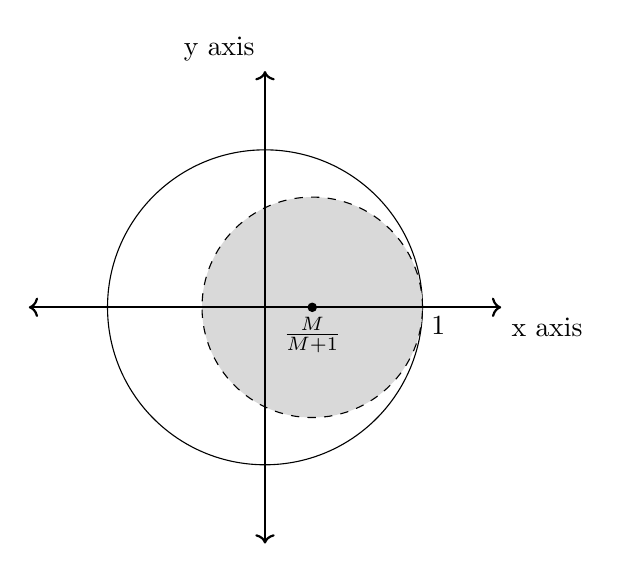
\begin{tikzpicture}	
	\draw[color=black] (0,0) circle [radius=2];
	\draw[black,fill=gray!30,dashed] (0.6,0) circle [radius=1.4];
	\filldraw[black] (0.6,0) circle (1.5pt);
	\draw (0.6,0) node[below]{$\frac{M}{M+1}$};
	\draw[thick,<->] (-3,0) -- (3,0)  node[anchor=north west] {x axis};
	\draw (2.2,0) node[below]{$1$};
	\draw[thick,<->] (0,-3) -- (0,3) node[anchor=south east] {y axis};		
\end{tikzpicture}

\end{document}